% compile using latex (xelatex seems to crop the figure strangely)
\documentclass{article} % For LaTeX2e
\usepackage[dvips]{graphicx}
\usepackage{nips14submit_e,times}
\usepackage{hyperref}
\usepackage{mdframed}
\usepackage{rotating}
\usepackage[outdir=./]{epstopdf}

\usepackage{graphics,graphicx}
\usepackage{amsmath,amssymb,amsfonts,comment}

\newcommand{\p}{\mathrm{P}}
\newcommand{\word}[1]{\texttt{#1}}
\newcommand{\mar}[1]{\marginpar{\footnotesize \bfseries
    \raggedright #1}}

\urldef{\googlegroup}\url{https://groups.google.com/forum/#!forum/word2vec-toolkit}
\urldef{\blogpost}\url{https://blog.lateral.io/2015/06/the-unknown-perils-of-mining-wikipedia/}

\title{Controlled Experiments for Word Embeddings}

 \author{
 	Benjamin Wilson\\
	Lateral GmbH\\
	\texttt{benjamin@lateral.io}
	\And
	Adriaan Schakel\\
	NNLP\\
	\texttt{adriaan.schakel@gmail.com}
 }

\date{\today}
\nipsfinalcopy % Uncomment for camera-ready version

\begin{document}

\graphicspath{{../outputs/}}
\maketitle

\begin{abstract}
	An experimental approach to studying the properties of word
        embeddings is proposed.  Controlled experiments, achieved
        through modifications of the training corpus, permit the
        demonstration of direct relations between word properties and
        word vector direction and length.  The new approach is
        demonstrated using the word2vec CBOW model with experiments that
        independently vary word frequency and word co-occurrence noise.
        The experiments reveal that word vector length depends more or
        less linearly on both word frequency and the level of noise in
        the co-occurrence distribution of the word.  The coefficients of
        linearity depend upon the word.
\end{abstract} 

\begin{section}{Introduction}
The field of natural language processing (NLP) is presently undergoing rapid
developments, not in the least triggered by the tremendous commercial
promises it holds.  A timely research topic in NLP are word embeddings,
where words from a vocabulary are represented by dense, real-valued
vectors.  Instead of one-hot vectors that merely indicate the location
of a word in the vocabulary, dense
vectors of dimension much smaller than the vocabulary size are
constructed such that they carry syntactic and semantic information.
Irrespective of the technique chosen, word embeddings are
typically derived from word co-occurrences.  More specifically, in a
machine-learning setting, word embeddings are typically trained by
scanning a short window over all the text in a corpus.  This process can
be seen as sampling word co-occurrence distributions, where it is
recalled that the co-occurrence distribution of a target word $w$
denotes the conditional probability $\p(w'|w)$ that a word $w'$ occurs in
its context, i.e., given that $w$ occurred.  Most applications of word
embeddings explore not the word vectors themselves, but relations
between them to solve, for example, similarity and word relation tasks
\cite{vecchi-baroni-zamparelli2011}.  For these tasks, it was found that using normalised word
vectors improves performance.  Word vector length is therefore typically
ignored.

In a previous paper \cite{schakel-wilson}, we proposed the use of word
vector length as measure of word significance.  Using a domain-specific
corpus of scientific abstracts, we observed that words that appear only
in similar contexts tend to have longer vectors than words of the same
frequency that appear in a wide variety of contexts.  For a given
frequency band, we found meaningless function words clearly separated
from proper nouns, each of which typically carries the meaning of a
distinctive context in this corpus.  In other words, the longer its
vector, the more significant a word is.  We also observed that word
significance is not the only factor determining the length of a word
vector, also the frequency with which a word occurs plays an important
role.

In this paper, we wish to study in detail to what extent these two
factors determine word vectors.  For a given corpus, both term
frequency and co-occurrence are, of course, fixed and it is not obvious
how to unravel these dependencies in an unambiguous, objective manner.
In particular, it is difficult to establish the distinctiveness of the
contexts in which a word is used.  To overcome these problems, we
propose to modify the training corpus in a controlled fashion.  To
this end, we insert new tokens into the corpus with varying frequencies
and varying levels of noise in their co-occurrence distributions.  By
modelling the frequency and co-occurrence distributions of these tokens
on existing words in the corpus, we are able to study their effect on
word vectors independently of one another.  We can thus study a family
of tokens that all appear in the same context, but with different
frequencies, or study a family of tokens that all have the same
frequency, but appear in a different number of contexts.  Starting from
the limited number of contexts in which a word appears in the original
corpus, we can increase this number by inspersing the word in arbitrary
contexts at random.  The word thus looses its significance in a
controlled way.  Although we present our approach using the word2vec
CBOW model, these and related experiments could equally well be carried
out for other word embedding methods such as the word2vec skip-gram
model \cite{DistRepns,EfficientEstimation}, GloVe
\cite{pennington2014glove}, and SENNA \cite{collobert-2011}.

We show that the length of the word vectors generated by the CBOW model
depends more or less linearly on both word frequency and level of noise
in the co-occurrence distribution of the word.  In both cases, the
coefficient of linearity depends upon the word.  If the co-occurrence
distribution is fixed, then word vector length increases with word
frequency.  If, on the other hand, word frequency is held constant, then
word vector length decreases as the level of noise in the co-occurrence
distribution of the word is increased.  We show furthermore that the
direction of the word vectors is independent of both word frequency and
co-occurrence noise.

This paper is structured as follows.  Section \ref{related-work} draws
connections to related work, while Section \ref{corpus-and-model} describes
the corpus and the CBOW model used in our experiments.
Section \ref{WFVE} describes a controlled experiment for varying word
frequency while holding the co-occurrence distribution fixed.
Section \ref{CNVE}, in a complementary fashion, describes a controlled
experiment for varying the level of noise in the co-occurrence
distribution of a word while holding the word frequency fixed.  The
final section, Section \ref{future-directions}, considers further questions
and possible future directions.
\end{section}

\begin{section}{Related work}\label{related-work}
Our notion of word significance is reminiscent of the concept of
``contextual distinctiveness'' introduced earlier by McDonald and
Shillcock \cite{mcdonald2001contextual}, who also based their work on word co-occurrences.
They define contextual distinctiveness of a target word $w$ as the
Kullback-Leibler divergence $\mathrm{D} \big(\p(w') ||\p(w'|w) \big)$
between the distribution of context words, $\p(w')$, and the
co-occurrence distributions of that target word $w$.  Specifically,
\begin{equation} 
\label{cd}
\mathrm{D} \big(\p(w') ||\p(w'|w) \big) = \sum_{w'} \p(w'|w) \log_2
\frac{\p(w'|w)}{\p(w')},
\end{equation} 
where the sum is over the set of \textcolor{blue}{content?} words $w'$.  They set the
window size to five words before and five words after the target word.
To reduce the computational burden, they recorded co-occurrences of 690
target words, randomly chosen from equally divided frequency bands, with
only the $n=500$ most frequent content words.  As pointed out by the
authors, contextual distinctiveness is a measure of the amount of
information provided by word $w$ about its contexts of use.  More specifically, if a
word $w$ tends to appear in a wide variety of contexts, the distribution
of the words it occurs with, i.e., the posterior distribution $\p(w'|w)$,
tends to diverge less from the prior distribution $\p(w')$, and its
contextual distinctiveness is accordingly small.  If, on the other hand,
$w$ typically appears in only a small number of different contexts, the
posterior distribution tends to diverge more from the prior, and a
larger value of contextual distinctiveness results.  As for
word significance, contextual distinctiveness summarizes a word's
contextual behavior in a single number. \textcolor{blue}{shorten?}

Our experimental finding that word vector length decreases with
co-occurrence noise is related to earlier work by Vecchi, Baroni, and
Zamparelli \cite{vecchi-baroni-zamparelli2011}, where a relation between
vector length and the ``semantic deviance'' of an adjective-noun
composite was studied empirically.  In that paper, which is also based
on word co-occurrence, the authors study adjective-noun composites.
They built a vocabulary from the 8k most frequent nouns and 4k most
frequent adjectives in a large general language corpus and added 22k
adjective-noun composites.  For each item in the vocabulary, they
recorded their co-occurrence within the same sentence with any of the
top 10k most frequent content words (nouns, adjectives or verbs) in the
corpus, and contructed word embeddings (of dimension 300) through
singular value decomposition of the co-occurrence matrix.  The authors considered several models for
constructing vectors of unattested adjective-noun composites, the two
simplest being adding and component-wise multipying the adjective and
noun vectors.  They hypothesized that the length of the vectors thus
constructed can be used to distinguish acceptable and semantically
deviant adjective-noun composites.  Using a few hundred adjective-noun
composites selected by humans for evaluation, they found that deviant
composites have a shorter vector than acceptable ones, in accordance
with their expectation.

In the word2vec similarity and word relationship tasks, normalised word vectors are used.
Word vector length is thus disregarded.
In the word2vec forum\footnote{\googlegroup}, it has been observed that normalisation improves performance on these tasks since word vector length is related to word frequency.
It remained unclear, however, whether word frequency was \textit{directly} related to word vector length or rather via correlated factors such as word significance.
Our experimental approach demonstrates that a direct relationship indeed exists.
It is shown moreover that the normalisation of the word vectors also prevents word co-occurrence noise from affecting the performance of the word similarity and word relationship tasks.

On the other hand, recent theoretical work \cite{Arora2015} has approached the problem of explaining the so-called ``compositionality'' property exhibited by some word embeddings.
In that work, unnormalised vectors are used in their model of the word relationship task.
It is hoped that experimental approaches such as those described here might enable theoretical investigations to describe the role of the word vector length in the word relationship tasks.
\end{section}

\begin{section}{Corpus and model}\label{corpus-and-model}
Our training data is built from the Wikipedia datadump from October
2013.  To remove the bulk of robot-generated pages from the training
data, only pages with at least 20 monthly page views are
retained.\footnote{For further justification and to obtain the dataset,
  see \blogpost} Stubs and disambiguation pages are also removed,
leaving 463 thousand pages with a total of 482 million words.
Punctuation marks and numbers were removed from the pages and all words
were lower-cased.  Word- (or ``term-'') frequency $tf$ is described in overview
in Table~\ref{word-occurrences-table}.  This base corpus is then
modified as described in Sections \ref{WFVE} and \ref{CNVE}.  For
recognisability, the tokens inserted into the corpus are upper-cased.

\begin{subsection}{Word2vec}\label{word2vec}
Word2vec, a feedforward neural network with a single hidden
layer, learns word vectors from word co-occurrences in an unsupervised
manner.  Word2vec comes in two versions.  In the continuous bag-of-words
(CBOW) model, the words appearing around a target word serve as input.
That input is projected linearly onto the hidden layer and the networks
then attempts to predict the target word on output.  Training is
achieved through backpropagation.  The word vectors are encoded in the
weights of the first synaptic layer, ``syn0''.  The weights of the
second synaptic layer (``syn1neg'', in the case of negative sampling) are typically discarded.  In the other model,
called skip-gram, target and context words swap places, so that the
target word now serves as input, while the network attempts to predict
the context words on output.

For simplicity only the word2vec CBOW word embedding with a single set
of hyperparameters is considered.  Specifically, a CBOW model with a
hidden layer of size 100 is trained using negative sampling with 5
negative samples, a window size of $10$, a minimum word occurrence of
$128$, and $10$ passes through the corpus.  Sub-sampling was not used so
that the influence of word frequency could be more clearly discerned.
Similar experimental results were obtained using hierarchical softmax,
but these are omitted for succinctness.  The relatively high
low-frequency cut-off is chosen to ensure that word vectors, in all but
degenerate cases, receive a sufficient number of gradient updates to be
meaningful.  This frequency cut-off results in a vocabulary of $81117$
words (only unigrams were considered).

The most recent revision of word2vec was used.\footnote{SVN revision 42,
  see \url{http://word2vec.googlecode.com/svn/trunk/}} The source code
for performing the experiments is made available on
GitHub.\footnote{\url{https://github.com/benjaminwilson/word2vec-norm-experiments}}

\begin{table}
	\begin{tabular}{c | r | l}
frequency band & \# words & example words  \\
\hline
$2^{0} - 2^{1}$ & 979187 & \word{isa220, zhangzhongzhu, yewell, gxgr} \\
$2^{1} - 2^{2}$ & 416549 & \word{wz132, prabhanjna, fesh, rudick} \\
$2^{2} - 2^{3}$ & 220573 & \word{gustafsdotter, summerfields, autodata, nagassarium} \\
$2^{3} - 2^{4}$ & 134870 & \word{futu, abertillery, shikaras, yuppy} \\
$2^{4} - 2^{5}$ & 90755 & \word{chuva, waffling, wws, andujar} \\
$2^{5} - 2^{6}$ & 62581 & \word{nagini, sultanah, charrette, wndy} \\
$2^{6} - 2^{7}$ & 41359 & \word{shew, düül, kidjo, strangeways} \\
$2^{7} - 2^{8}$ & 27480 & \word{smartly, sydow, beek, falsify} \\
$2^{8} - 2^{9}$ & 17817 & \word{legionaries, möbius, mannerism, cathars} \\
$2^{9} - 2^{10}$ & 12291 & \word{bedtime, disabling, jockeys, brougham} \\
$2^{10} - 2^{11}$ & 8215 & \word{frederic, monmouth, constituting, grabbing} \\
$2^{11} - 2^{12}$ & 5509 & \word{questionable, bosnian, pigment, coaster} \\
$2^{12} - 2^{13}$ & 3809 & \word{dismissal, torpedo, coordinates, stays} \\
$2^{13} - 2^{14}$ & 2474 & \word{liberty, hebrew, survival, muscles} \\
$2^{14} - 2^{15}$ & 1579 & \word{destruction, trophy, patrick, seats} \\
$2^{15} - 2^{16}$ & 943 & \word{draft, wood, ireland, reason} \\
$2^{16} - 2^{17}$ & 495 & \word{brought, move, sometimes, away} \\
$2^{17} - 2^{18}$ & 221 & \word{february, children, college, see} \\
$2^{18} - 2^{19}$ & 83 & \word{music, life, following, game} \\
$2^{19} - 2^{20}$ & 29 & \word{during, time, other, she} \\
$2^{20} - 2^{21}$ & 17 & \word{has, its, but, an} \\
$2^{21} - 2^{22}$ & 10 & \word{by, on, it, his} \\
$2^{22} - 2^{23}$ & 4 & \word{was, is, as, for} \\
$2^{23} - 2^{24}$ & 3 & \word{in, and, to} \\
$2^{24} - 2^{25}$ & 1 & \word{of} \\
$2^{25} - 2^{26}$ & 1 & \word{the} \\
\end{tabular}

	\caption{ Number of words, by frequency band, as observed in the
          unmodified corpus.  }
	\label{word-occurrences-table}
\end{table}
\end{subsection}

\begin{subsection}{Replacement procedure}\label{replacement-procedure}
In the experiments detailed below, we modify the corpus in a controlled
manner by introducing tokens into the corpus via a replacement procedure
as follows.  Consider a word, say \word{cat}.  For each occurrence of
this word, a sample $i$, $1 \leqslant i \leqslant n$ is drawn from a
truncated geometric distribution, and that occurrence of the word
\word{cat} is replaced with the token \word{CAT\_i}.  In this way, the
word \word{cat} is replaced throughout the corpus by a family of tokens
with varying frequencies but approximately the same co-occurrence
distribution as \word{cat}.  That is, all these tokens are used in
roughly the same contexts as the original word.

The geometric distribution is truncated in order to limit the number of
tokens inserted into the corpus.  For any choice $0 < p < 1$ and
maximum value $n > 0$, the truncated geometric distribution is given by
the probability density function
\begin{equation} 
\label{distro}
P_{p, n} (i) = \frac{p^{i-1}  (1-p)}{1 - p^n}, \qquad 1
\leqslant i \leqslant n.
\end{equation} 
The factor in the denominator, which tends to unity in the limit $n \to
\infty$, assures proper normalisation.  We have chosen this distribution
because the probabilities decay exponentially base $p$ as a function of
$i$.  Of course, other distributions might equally well have been chosen
for the experiments.
\end{subsection}
\end{section}

\begin{section}{Varying word frequency}\label{WFVE}
In this first experiment, we investigate the effect of word frequency on
the word embedding.  Using the replacement procedure, we introduce a
small number of families of tokens into the corpus.  The tokens in each
family vary in frequency but, replacing a single word, all share a
common co-occurrence distribution.  This allows us to study the role of
word frequency in isolation, everything else being kept equal.  We
consider two types of tokens.

\begin{subsection}{Tokens derived from existing words}\label{WFVEexisting}
%
We choose uniformly at random a small number of words from the
unmodified vocabulary for our experiment.  In order that the inserted
tokens do not have too low a frequency, only words which occur at least
10 thousand times are chosen.  We also include the high-frequency
stopword \word{the} for comparison.  Table~\ref{word-frequency-counts}
lists the words chosen for this experiment along with their frequencies.

The replacement procedure of Section ~\ref{replacement-procedure} is then
performed for each of these words, using a geometric decay rate of $p =
\tfrac{1}{2}$, and maximum value $n=20$, so that the 1st token is
inserted with a probability of about $0.5$, the 2nd with a probability of
about $0.25$, and so on.  This value of $p$ is one of a range of values
that ensure that, for each word, multiple tokens will be inserted with a
number of occurrences sufficient to survive the low-frequency cut-off of
128.  A maximum value $n=20$ suffices for this choice of $p$, since
$2^{20 + \log_2{128}}$ exceeds the maximum occurrence count of any token in
the corpus.  Figure~\ref{fig:word-frequency-experiment-text-cat}
illustrates the effect of these modifications on a sample text, with a
family of tokens \word{CAT\_i}, derived from the word \word{cat}.
Notice that all occurences of the word \word{cat} have been replaced
with the tokens \word{CAT\_i}.

\begin{table}
	\begin{center}
\begin{tabular}{l | r}
word & frequency \\
\hline
\word{lawsuit} & 11565 \\
\word{mercury} & 13059 \\
\word{protestant} & 13404 \\
\word{hidden} & 15736 \\
\word{squad} & 24872 \\
\word{kong} & 32674 \\
\word{awarded} & 55528 \\
\word{response} & 69511 \\
\word{the} & 38012326 \\
\end{tabular}
\end{center}

	\caption{Term frequency $tf$ of words chosen for the word
          frequency experiment. }
	\label{word-frequency-counts}
\end{table}

\begin{figure}
	\begin{mdframed}
	\texttt{the domestic \textcolor{red}{CAT\_1} was first classified as felis catus\newline the semiferal \textcolor{red}{CAT\_1} a mostly outdoor \textcolor{red}{CAT\_1} is not owned by any one individual\newline a pedigreed \textcolor{red}{CAT\_1} is one whose ancestry is recorded by a \textcolor{red}{CAT\_2} fancier organization\newline a purebred \textcolor{red}{CAT\_1} is one whose ancestry contains only individuals of the same breed\newline the \textcolor{red}{CAT\_1} skull is unusual among mammals in having very large eye sockets\newline another unusual feature is that the \textcolor{red}{CAT\_3} cannot produce taurine\newline within groups one \textcolor{red}{CAT\_3} is usually dominant over the others}
	\end{mdframed}
	\caption{Example sentences modified in the word frequency
          experiment as per Section ~\ref{WFVEexisting}, where the word
          \word{cat} is replaced with tokens \word{CAT\_i} using the
          truncated geometric distribution (\ref{distro}) with
          $p=\tfrac{1}{2}$ and $n=20$.}
	\label{fig:word-frequency-experiment-text-cat}
\end{figure}

\end{subsection}

\begin{subsection}{Tokens derived from an artificial, meaningless word}\label{WFVEmeaningless}
%
Whereas the tokens introduced above all replace an existing word that
carries a meaning, we now include for comparison a high-frequency,
meaningless word.  We choose to introduce an artificial, entirely
meaningless word \word{VOID} into the corpus, rather than choose an
existing (stop)word whose meaninglessness is only supposed.  To achieve
this, we insperse the word uniformly at random throughout the corpus so
that its global frequency is $0.005$.  The co-occurrence
distribution of \word{VOID} thus coincides with the global word
distribution.  The replacement procedure is then performed for this
word, using the same values for $p$ and $n$ as above.
Figure~\ref{fig:word-frequency-experiment-text-void} shows the effect of
these modifications on a sample text, where a higher global frequency of $0.05$ is used instead
for illustrative purposes.  Although the probability of inserting token
\word{VOID\_1} is twice that of iserting token \word{VOID\_2} and four
times that of inserting token \word{VOID\_3}, these three tokens all
appear once in this small piece of text.

\begin{figure}
	\begin{mdframed}
	\texttt{the domestic cat was first classified as felis catus\newline the semiferal cat a mostly outdoor cat is not owned by any one individual\newline a pedigreed cat is one whose ancestry is recorded by a cat fancier organization\newline a purebred cat is one whose ancestry contains only individuals of the same breed\newline the cat skull is unusual among mammals in having very large eye sockets\newline another unusual feature is that the cat cannot produce taurine\newline \textcolor{red}{VOID\_1} within groups one cat is usually dominant over the others}
	\end{mdframed}
	\caption{The same example sentences as in
          Figure ~\ref{fig:word-frequency-experiment-text-cat} where
          instead of the word \word{cat} now the meaningless word
          \word{VOID} is replaced with tokens \word{VOID\_i}.  For
          illustrative purposes, the meaningless word \word{VOID} was
          here interspersed with a global frequency of $0.05$.}
	\label{fig:word-frequency-experiment-text-void}
\end{figure}
\end{subsection}

\subsection{Experimental results}
We next present the results of the word frequency experiment. We
consider the effect of word frequency on the direction and on the length
of word vectors separately.

\subsubsection{Word frequency and vector direction}\label{WFVE-direction}
%
Figure~\ref{word-frequency-experiment-heatmap} shows the cosine
similarity of pairs of vectors representing some of the tokens used in
this experiment.  Recall that the cosine similarity measures the extent
to which two vectors have the same direction, taking a maximum value of
$1$ and a minimum value of $-1$.  The number of different tokens
associated with an experiment word is the number of times that its
frequency can be halved and remain above the low-frequency cut-off of
$128$.

Consider first the words other than \word{the} and \word{VOID}.  These
words typically occur in a limited number of distinct contexts, and
so a limited number of samples is required to capture their
co-occurrence distributions.  We therefore expect that the vectors
representing the tokens derived from any of these words can be properly
learned from the modified corpus, even though their combined number of
occurences equals the term frequency of that word in the original
corpus.  The red blocks in Figure ~\ref{word-frequency-experiment-heatmap}
clearly demonstrate that the direction of these vectors is constant for
each family of tokens.  In other words, the direction of these vectors
is only determined by the original word and is independent of how often
that words appear, provided sufficient samples have been processed for
the word vector to settle in its equilibrium direction.

The artificial word \word{VOID}, on the other hand, occurs by
construction in every context.  A much higher number of samples is
therefore required to capture its co-occurrence distribution, and
thereby to learn its word vector.  The same is true, but to a lesser
extent, for the stopword \word{the}.  The difficulty of learning the
vector representing \word{VOID\_i} or \word{THE\_i} increases with $i$,
for the tokens occur increasingly less often.  This is consistent with
Figure ~\ref{word-frequency-experiment-heatmap}, where it is apparent that
the vectors representing \word{VOID\_i} for small $i$, say $i = 1,
\dots, 5$, roughly share a common direction, while this is no longer
true for higher values of $i$.  The same trend is apparent, although
less extremely so, for the word \word{the}.  The vectors for the tokens
\word{THE\_i} share a common direction for values of $i$ as high as
$14$, before they start changing direction.  We conclude that these
deviations are artifacts of poor learning due to an insufficient number
of occurrences of these tokens.
Table~\ref{word-frequency-experiment-cosine-similarity}, showing the
most similar words to each token \word{THE\_i}, supports this further.  In the
discussions below, the tokens \word{VOID\_i} and
\word{THE\_i} whose vectors have a cosine similarity less than $0.8$
with \word{VOID\_1} and \word{THE\_1}, respectively are therefore
discarded.

From these results, we conclude that word frequency has no effect on the
direction of a word vector, given a sufficient number of samples to
learn the co-occurrence distribution of the word.
%For well-learned representations, word frequency has no effect on word
%vector direction.

\subsubsection{Word frequency and vector length}
%
We next consider the effect of frequency on word vector length.
Figure~\ref{fig:word-frequency-experiment-graph} shows this relation for
individual words, both for the word vectors, represented by the weights
of the first synaptic layer, syn0, in the word2vec neural network, and
for the vectors represented by the weights of the second synaptic layer,
syn1neg.  We include the latter, which are typically ignored, for
completeness.  Each line corresponds to a single word, and the points on
each line indicate the frequency and vector length of the tokens derived
from that word.  For example, the six points on the line corresponding
to the word \word{protestant} are labeled, from right to left, by the
tokens \word{PROTESTANT\_1}, \word{PROTESTANT\_2}, \dots,
\word{PROTESTANT\_6}.  Again, the number of points on the line is
determined by the frequency of the original word.  For example, the
frequency of the word \word{protestant} can be halved at most $6$ times
so that the number of occurences of the last token is still above the
low-frequency cut-off.  Because all the points on a line share the same
co-occurrence distribution, the left panel in
Figure ~\ref{fig:word-frequency-experiment-graph} demonstrates conclusively
that length does indeed depend on frequency directly.  Moreover, this
relation is seen to be approximately linear for each word considered.
Notice also that the relative positions of the lengths of the word vectors associated
with the experiment words are roughly independent of the frequency band,
i.e., the plotted lines rarely cross.

Notice the inflection of the syn1neg curve in
Figure ~\ref{fig:word-frequency-experiment-graph} for \word{the} at
approximately $tf=10^6$.  We have no explanation of this.  Also observe
that the lengths of the vectors representing the meaningless tokens
\word{VOID\_i} are approximately constant.  Since we already found the
direction to be also constant, it is sensible to speak of the word
vector of \word{VOID} irrespective of its frequency.  In particular, the
token \word{VOID\_1} may be taken as an approximation.

\begin{figure}
	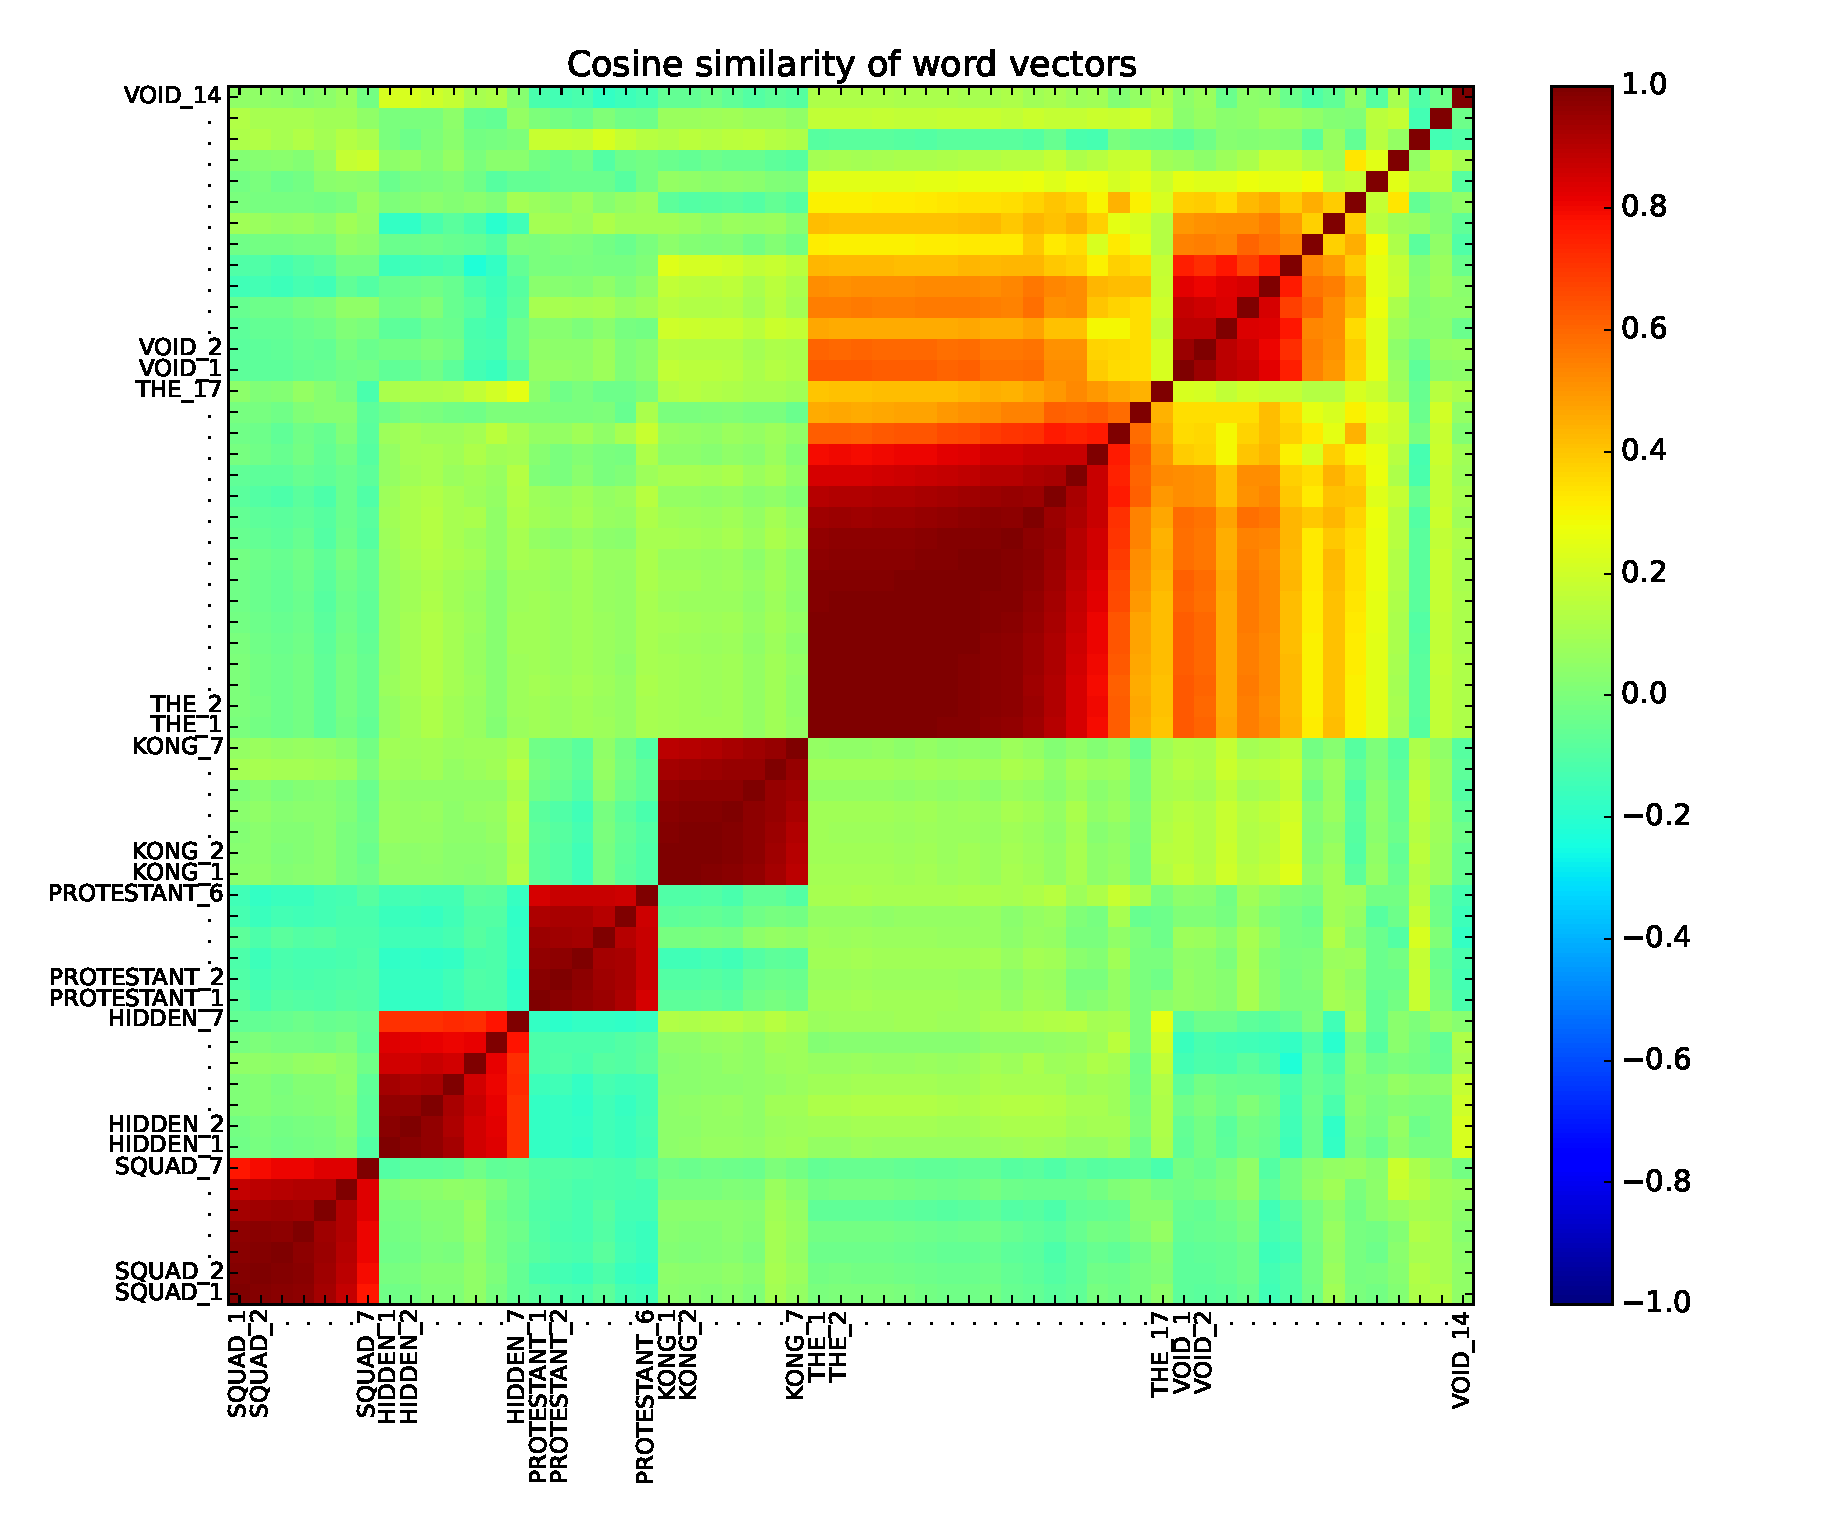
\includegraphics[scale=0.5]{word-frequency-experiment-heatmap}
	\caption{ Heatmap of the cosine similarity of the vectors
          representing some of the tokens used in the word frequency
          experiment.  The words other than \word{the} and \word{VOID}
          were chosen randomly.  }
	\label{word-frequency-experiment-heatmap}
\end{figure}

\begin{table}
	\begin{tabular}{l | c | l}
token & similarity to \word{THE\_1} & most similar words in unmodified corpus\\
\hline
\word{THE\_1} & 1.0000 & \word{this, its, another, whose} \\
\word{THE\_2} & 0.9994 & \word{this, its, another, whose} \\
\word{THE\_3} & 0.9989 & \word{this, its, another, ii} \\
\word{THE\_4} & 0.9988 & \word{this, its, another, whose} \\
\word{THE\_5} & 0.9983 & \word{this, its, another, integrally} \\
\word{THE\_6} & 0.9967 & \word{this, its, another, ii} \\
\word{THE\_7} & 0.9920 & \word{this, its, another, ii} \\
\word{THE\_8} & 0.9879 & \word{this, its, another, whose} \\
\word{THE\_9} & 0.9776 & \word{this, its, another, integrally} \\
\word{THE\_10} & 0.9672 & \word{this, its, ii, another} \\
\word{THE\_11} & 0.9460 & \word{this, its, ii, another} \\
\word{THE\_12} & 0.9110 & \word{this, its, another, ii} \\
\word{THE\_13} & 0.8704 & \word{this, its, another, ii} \\
\word{THE\_14} & 0.7730 & \word{ii, this, another, multi} \\
\word{THE\_15} & 0.7043 & \word{lengthy, rassilon, of, veritable} \\
\word{THE\_16} & 0.5107 & \word{initiated, projected, gradual, marking} \\
\word{THE\_17} & 0.2762 & \word{texcoco, castrum, uqba, bouillon} \\
\word{THE\_18} & 0.2074 & \word{revolved, presided, revolves, revolving} \\
\end{tabular}

	\caption{ Words in the original vocabulary most similar to the
          tokens \word{THE\_i}, and their cosine similarity with the
          most frequent such token, \word{THE\_1}.  It is apparent from
          the nearest neigbour list that the vectors of the
          low-frequency tokens have not been adequately trained.  }
	\label{word-frequency-experiment-cosine-similarity}
\end{table}

\begin{sidewaysfigure*}
	\centering{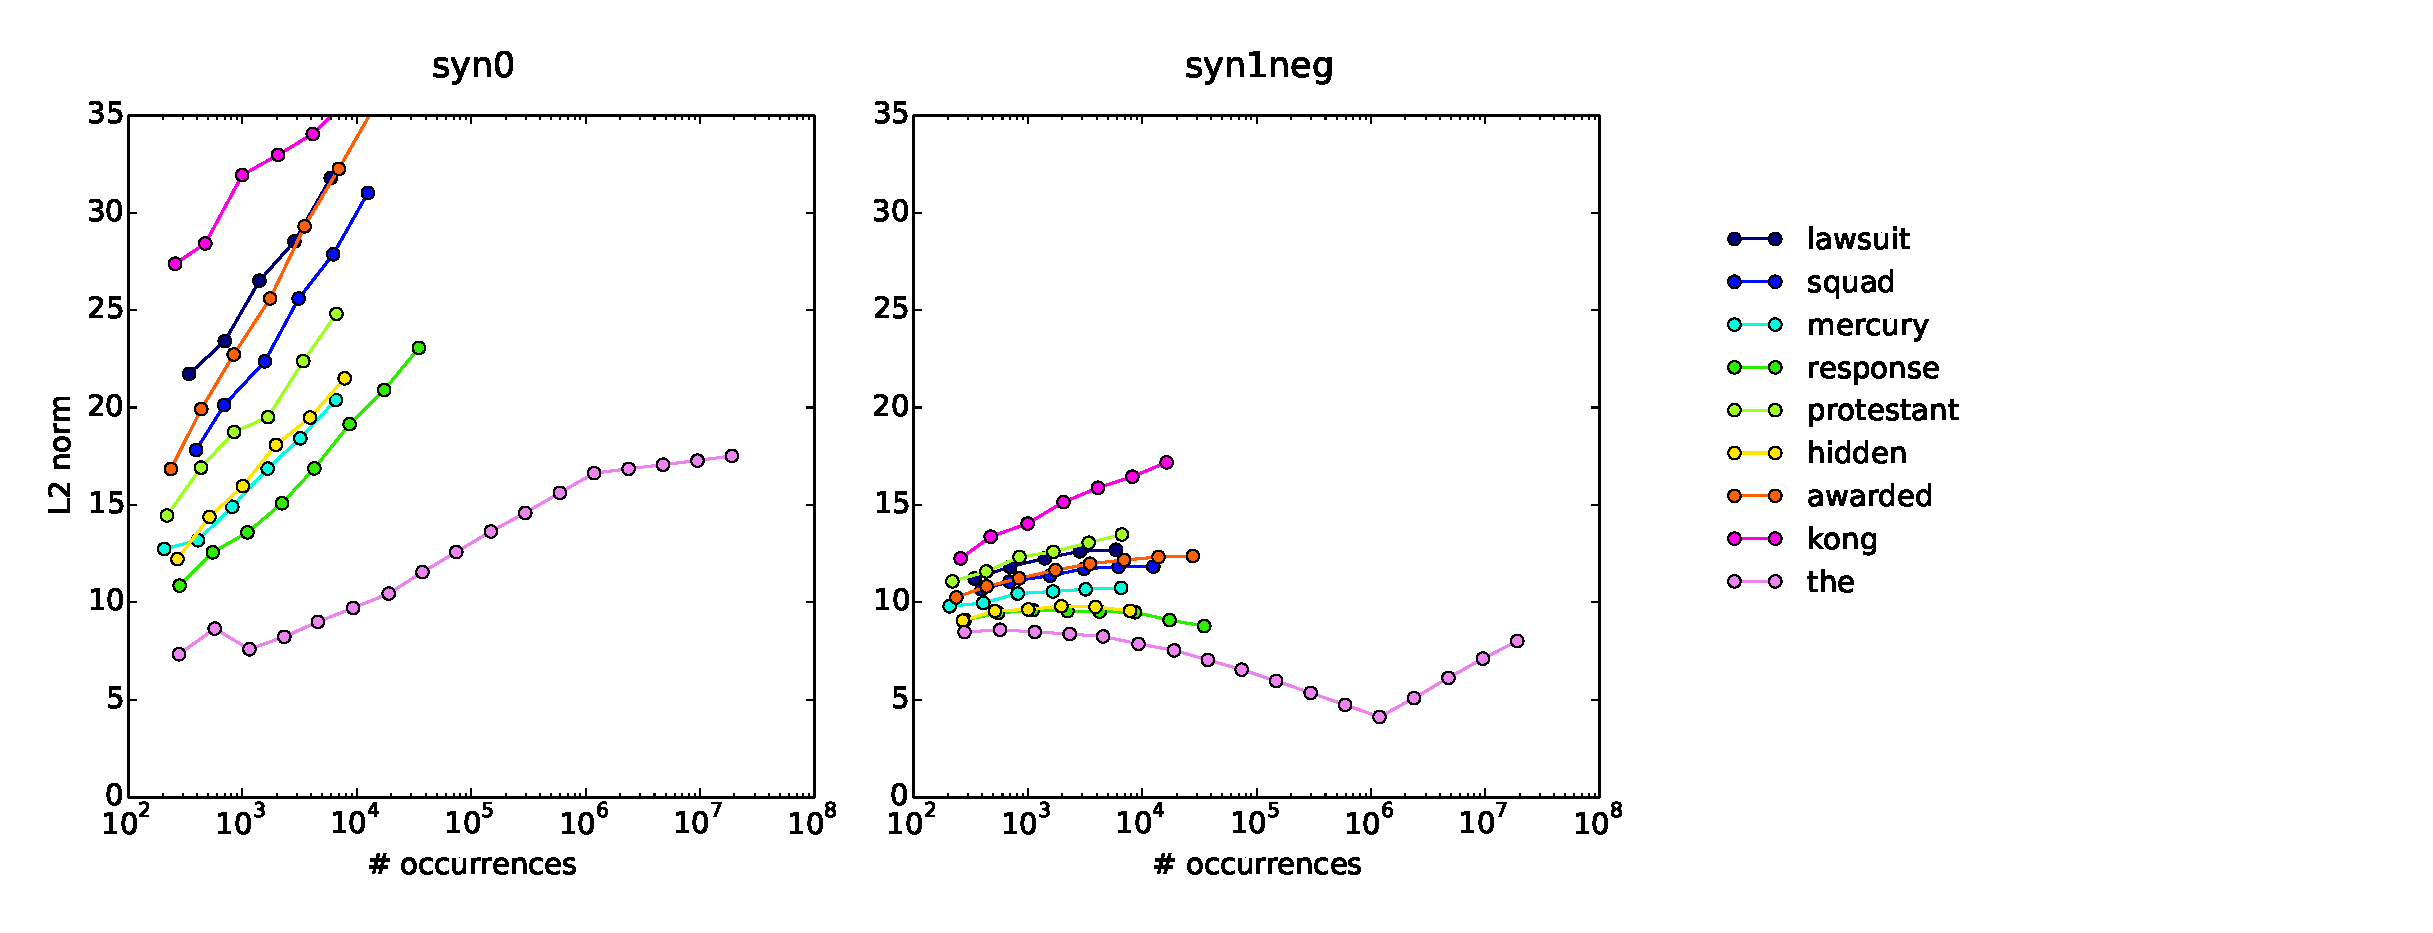
\includegraphics[scale=0.6]{word-frequency-experiment-graph}}
	\caption{ Vector length vs. frequency for tokens derived from a
          few words chosen at random.  For each word, tokens of varying
          frequency but with the co-occurrence distribution of that word
          were inserted into the corpus, as described in
          Section ~\ref{WFVE}.  The vectors are obtained from the first
          synaptic layer, syn0, of the word2vec neural network.  The
          vectors obtained from the second layer, syn1neg, are
          included for completeness.  }
	\label{fig:word-frequency-experiment-graph}
\end{sidewaysfigure*}
\end{section}

\begin{section}{Varying co-occurrence noise}\label{CNVE}
This second experiment is complementary to the first.  Wheras in the
first experiment we studied the effect of word frequency on word vectors
for fixed co-occurence, we next study the effect of co-occurence for
fixed frequency.
  
\subsection{Generating noise}
We do so again in a controlled manner by adding noise to the
co-occurence distribution.  We take the noise distribution to be the
global word distribution, so that noise can be simply added to the
co-occurrence distribution of a word by interspersing occurrences of
that word uniformly at random throughout the corpus.  A word that is
consistently used in a distinctive context in the unmodified corpus thus
appears in the modified corpus also in completely unrelated contexts.
As in Section \ref{WFVE}, we choose a small number of words from the
unmodified corpus for this experiment.  Table
\ref{cooccurrence-noise-words} lists the words chosen, along with their
frequencies in the corpus.

For each of these words, the replacement procedure of Subsection
\ref{replacement-procedure} is performed using a geometric rate of decay
of $p = \tfrac{5}{6}$, and truncating the distribution at $n=8$.  For
every replacement token (e.g. \word{CAT\_i}), occurrences of this
token are subsequently interspersed uniformly at random throughout the
corpus, such that the frequency of the replacement token is restored to
that of the original word \word{cat}.  For example, if the original word
\word{cat} occurred $1000$ times, then after the replacement procedure,
\word{CAT\_2} occurs approximately $694$ times, so a further
(approximately) $306$ random occurrences of \word{CAT\_2} are
interspersed throughout the corpus.  Thus the word \word{cat} is removed
from the corpus, and a family of tokens \word{CAT\_i}, $1 \leqslant i
\leqslant 8$ is introduced.  These tokens all have the same frequency as
the word \word{cat}, but their co-occurrence distributions, while based
on that of \word{cat}, have an increasing amount of noise.

Figure \ref{fig:co-occurrence-noise-experiment-text} illustrates the
effect of this modification in the case where the only word chosen is
\word{cat}.  The original text in this case concerned both cats and
dogs.  Notice that the word \word{cat} has been replaced entirely in the
cats section by \word{CAT\_i} and, moreover, that these same tokens
appear also in the dogs section. These occurrences (and additionally,
with probability, some occurrences from the cats section) constitute
noise.

The proportion of occurrences of the token \word{CAT\_i} that arise by
replacing the word \word{cat} is $P_{5/6, 8}(i)$, and the proportion
that arise from randomly interspersing this token throughout the corpus
is $r_i := 1 - P_{5/6, 8}(i)$.  The particular value of $p$ (large
compared to that of section \ref{WFVE}) was chosen so that the
proportion of noise $r_i$ did not increase too quickly with $i$.  These
proportions are the sampling points on our axis of variation, and this
value of $p$ (together with the choice of $n$) assures a reasonable
spread.  Other parameter values (or indeed other distributions) could,
of course, have been used equally well.

\begin{table}
	\begin{center}
\begin{tabular}{l | r}
word & \# occurrences \\
\hline
\word{dying} & 10693 \\
\word{bridges} & 12193 \\
\word{appointment} & 12546 \\
\word{aids} & 13487 \\
\word{boss} & 14105 \\
\word{removal} & 15505 \\
\word{jobs} & 21065 \\
\word{community} & 115802 \\
\end{tabular}
\end{center}

	\label{fig:co-occurrence-noise-counts}
	\caption{Term frequency $tf$ of words chosen for the
          co-occurrence noise experiment. }
	\label{cooccurrence-noise-words}
\end{table}

\begin{figure}
	\begin{mdframed}
	\texttt{the domestic \textcolor{red}{CAT\_2} was first classified as felis catus\newline the semiferal \textcolor{red}{CAT\_3} a mostly outdoor \textcolor{red}{CAT\_4} is not \textcolor{red}{CAT\_2} owned by any one individual\newline a pedigreed \textcolor{red}{CAT\_4} is one whose ancestry is recorded by a \textcolor{red}{CAT\_1} fancier organization\newline \textcolor{red}{CAT\_6} a purebred \textcolor{red}{CAT\_3} is one whose ancestry contains only individuals of the same breed\newline the \textcolor{red}{CAT\_1} skull is unusual among mammals in having very \textcolor{red}{CAT\_4} large eye sockets\newline another unusual feature is that the \textcolor{red}{CAT\_4} cannot produce taurine\newline within groups one \textcolor{red}{CAT\_2} is usually dominant over the others\newline ...\newline the domestic dog canis lupus familiaris is a domesticated canid which has been selectively \textcolor{red}{CAT\_5} bred\newline dogs perform many roles for people such as hunting herding and pulling loads\newline \textcolor{red}{CAT\_7} in domestic dogs sexual maturity begins to happen around age six to twelve months\newline this is \textcolor{red}{CAT\_6} the time at \textcolor{red}{CAT\_3} which female dogs will have their first estrous cycle\newline some dog breeds have acquired traits through selective breeding that interfere with reproduction}
	\end{mdframed}
	\caption{Example sentences modified for the co-occurrence noise
          experiment, where the word \word{cat} was chosen for
          replacement.  The tokens were generated using the distribution
          (\ref{distro}) with $p = \tfrac{5}{6}$ and $n=3$.}
	\label{fig:co-occurrence-noise-experiment-text}
\end{figure}

\begin{subsection}{Experimental results}
Figure~\ref{fig:co-occurrence-noise-heatmap} shows the cosine similarity
of pairs of vectors representing some of the tokens used in this
experiment.  The figure clearly demonstrates that vectors representing
tokens derived from the same word all share a common direction.  This
brings us to the conclusion that co-occurrence noise has no discernable effect on
the direction of word vectors.

%While the word2vec neural network
%samples co-occurrence noise, the direction of the vector representing
%the target word changes, but these changes cancel out, so that the
%direction remains fixed on average.

The left panel in Figure ~\ref{fig:co-occurrence-noise-graph}, on the other hand, reveals that vector length varies more or less
linearly with the proportion $r$ of noise in the co-occurrence
distribution.  This figure motivates our interpretation of vector
length, within a sufficiently narrow frequency band, as a measure of the
absence of co-occurrence noise, or put differently, of the extent to
which a word carries the meaning of a distinctive context.

When read from right to left, this figure can be reinterpreted and
related to the corresponding figure in
Figure ~\ref{fig:word-frequency-experiment-graph} as follows.  The
co-occurrence noise we generated appears to be white noise whose effects
cancel out on average.  The horizontal axis can then be reinterpreted as
denoting term frequency and a similar picture as in
Figure ~\ref{fig:word-frequency-experiment-graph} emerges, namely that the
word vector length increases more or less linearly with term frequency.
This can, however, not be the complete picture, for the vectors
represented by the second synaptic layer, syn1neg, show a different
behavior in the two figures.  In particular, the length of these vectors
is seen from the right panel of Figure ~\ref{fig:co-occurrence-noise-graph}
to be completely insensitive to noise, i.e., frequency in our
reinterpretation, whereas the length of those shown in the right panel
of Figure ~\ref{fig:word-frequency-experiment-graph} does depend on
frequency.

In this experiment, the introduced tokens are intermediate points on a path in the space of distributions over the vocabulary, beginning at the co-occurrence distribution of the word and ending at the global word frequency distribution, i.e. the co-occurrence distribution of \word{VOID}.
Thus it is clear a priori that the word vectors for the introducted tokens are intermediate steps on a path from the word vector of the original word to that of \word{VOID} (recall from \ref{WFVE} that its vector is approximately independent of its frequency).
While we observe from Figure \ref{fig:co-occurrence-noise-heatmap} that the word vectors for the tokens introduced for a word all share a common direction, this is only true to the extent that the word vector for \word{VOID} is close to zero.

\begin{figure}
	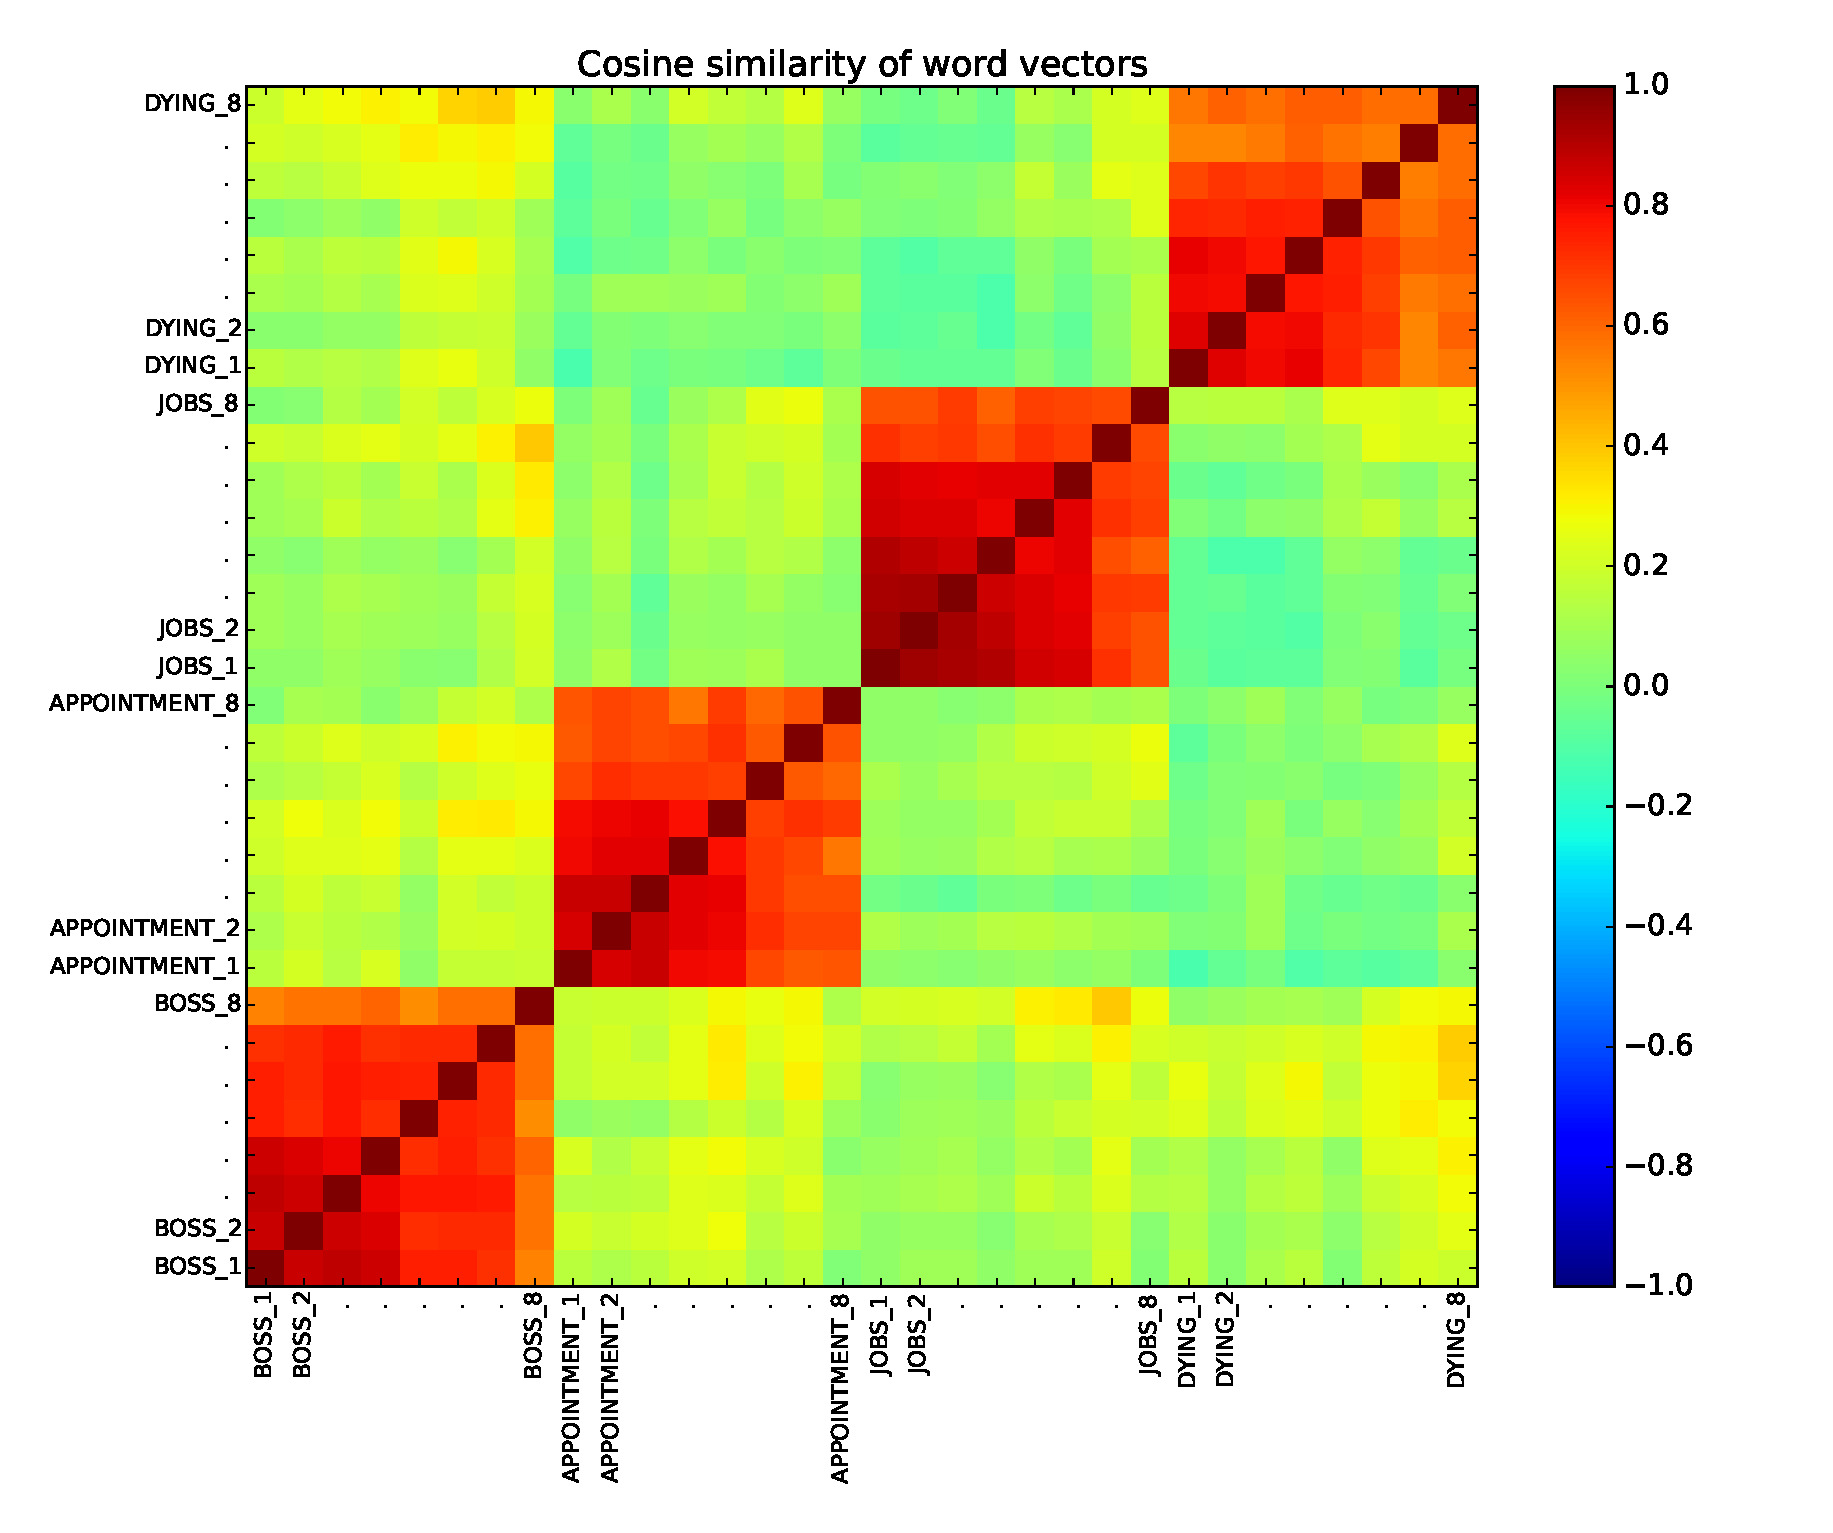
\includegraphics[scale=0.5]{cooccurrence-noise-heatmap}
	\caption{ Heatmap of the cosine similarity of the vectors
          representing some of the tokens used in the co-occurrence
          noise experiment (the words were chosen at random).  The
          largely red blocks demonstrate that the direction of the word
          vectors does not change when noise is added to the
          co-occurrence distribution.  }
	\label{fig:co-occurrence-noise-heatmap}
\end{figure}

\begin{sidewaysfigure*}
	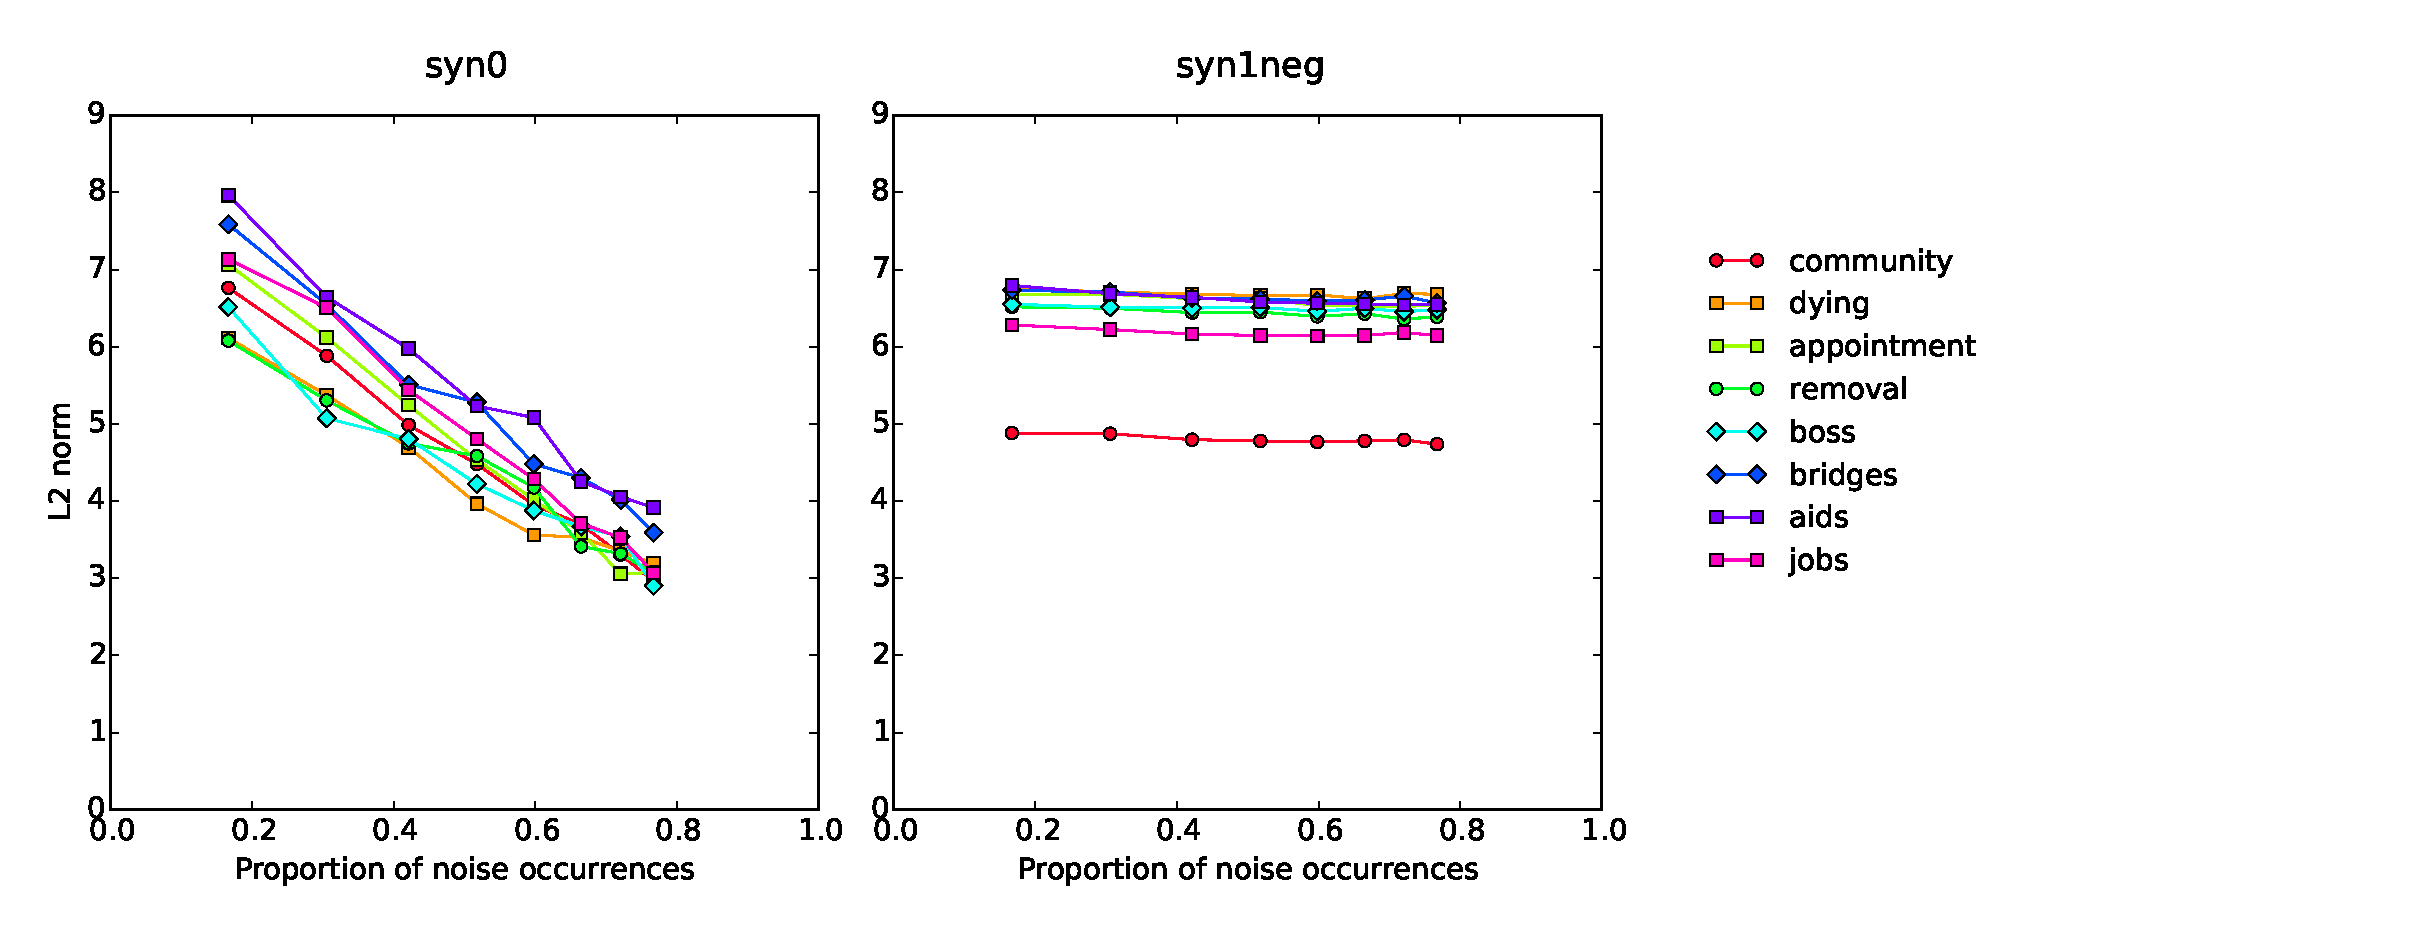
\includegraphics[scale=0.6]{cooccurrence-noise-graph}
	\caption{ Vector length vs. proportion of co-occurrence noise
          for words chosen for this experiment.  For each word, tokens
          of equal frequency but with increasing proportion of
          co-occurrence noise were inserted into the corpus, as
          described in section \ref{CNVE}.  The word vectors are
          obtained from the first synaptic layer, syn0.  The second
          layer, syn1neg, is included for completeness.  }
	\label{fig:co-occurrence-noise-graph}
\end{sidewaysfigure*}

\end{subsection}

\end{section}


\begin{section}{Discussion}\label{future-directions}

\begin{subsection}{Controlled experiments for word embeddings}
Our principle contribution has been to demonstrate that controlled experiments can be used to gain insight into a word embedding.
Because they are achieved via modification of the training corpus, these experiments can be carried out for any word embedding (or indeed language model), requiring no knowledge or modification of the model implementation.

It would, of course, be interesting to perform these experiments for other word embeddings other than word2vec CBOW and for different hyperparameters settings.

More elaborate experiments could be carried out.
For instance, by introducing tokens into the corpus that mix, with varying proportions, the co-occurrence distributions of two words, the path between the word vectors in the feature space could be studied.
The co-occurrence noise variation experiment described here would be a special case of such an experiment where one of the two words was \word{VOID}.
\end{subsection}

\begin{subsection}{Applications in other contexts}
Further afield, it would be interesting to perform analogs of these experiments in other contexts where models are trained from co-occurrence data.
For instance, in the context of e-Commerce, product purchase frequency and product co-occurrence noise can be varied by modifying the product-product co-occurrence matrix.
\end{subsection}

\begin{subsection}{Questions pertaining to word2vec}
Questions pertaining to word2vec in particular arise naturally from the results of the experiments.
Figures \ref{fig:word-frequency-experiment-graph} and \ref{fig:co-occurrence-noise-graph}, for example, demonstrate the word vectors obtained from the first synaptic layer, ``syn0'', have very different properties from those that could be obtained from the second layer, ``syn1neg'', which are typically discarded.
These differences warrant further investigation.

The co-occurrence distribution of \word{VOID} is the global frequency distribution, and in this sense pure background noise.
Thus the word vector of \word{VOID} is a special point in the feature space.
Figure \ref{fig:word-frequency-experiment-graph} shows that this point is not at the origin of the feature space (i.e. is not the zero vector).
The origin, however, is implicitly the point of reference in the word2vec word similarity task.
This raises the question of whether improved performance on the similarity task could be achieved by transforming the feature space (or modifying the model) such that the representation of pure noise (i.e. the vector for \word{VOID}) is at the origin of the transformed feature space. 

%\textcolor{red}{can it be argued that the feature space must be fundamentally euclidean, given that the path marked by the vectorisations of intermediate words is a straight line? i.e. if such paths maybe considered as ``geodesics'' between words, and we show that these geodesics appear as straight lines when an euclidean metric is imposed, then suggests that the euclidean metric is in fact a good choice.  what would happen if we chose another metric?}

\end{subsection}

\end{section}

\clearpage
\footnotesize
\bibliography{main}
\bibliographystyle{plain}
\end{document}
